\documentclass[10pt]{article}
\usepackage[verbose, a4paper, hmargin=2.5cm, vmargin=2.5cm]{geometry}

\usepackage{fontspec}
\usepackage{ctex}
\usepackage{paratype}

\usepackage{amsmath}
\usepackage{amssymb}
\usepackage{amsfonts}
\usepackage{esint}
\usepackage{stmaryrd}

\usepackage[mathbf=sym]{unicode-math}
\setmainfont{STIX Two Text}
\setmathfont{STIX Two Math}

\setsansfont{Arial}
\setmonofont{Courier New}

\usepackage{makecell}
\usepackage{wasysym}
\usepackage{pifont}
\usepackage[export]{adjustbox}
\usepackage{graphicx}
\usepackage{mdframed}
\usepackage{booktabs,array,multirow}
\usepackage{tabularx}
\usepackage{hyperref}
\hypersetup{colorlinks=true, linkcolor=blue, filecolor=magenta, urlcolor=cyan,}
\urlstyle{same}
\usepackage[most]{tcolorbox}
\definecolor{mygray}{RGB}{240,240,240}
\tcbset{
  colback=mygray,
  boxrule=0pt,
}
\graphicspath{ {./images/} }
\newcommand{\HRule}{\begin{center}\rule{0.9\linewidth}{0.2mm}\end{center}}
\newcommand{\customfootnote}[1]{
  \let\thefootnote\relax\footnotetext{#1}
}
\newcommand{\lt}{\mathrel{<}}
\newcommand{\gt}{\mathrel{>}}
\newcommand*\circled[1]{\tikz[baseline=(char.base)]{\node[shape=circle,draw,inner sep=1.5pt] (char) {\small #1};}}
\setcounter{MaxMatrixCols}{256}
\begin{document}
\section*{2026 届上海市奉贤区高三数学二模}

\begin{center}

\includegraphics[max width=1.0\textwidth]{images/bo_d7ci9kqlb0pc73de9leg_0_0_1_1374_2337_0.jpg}
\end{center}
\hspace*{3em} 

\section*{一、填空题(本题共 12 小题，1-6 每小题 4 分，7-12 每小题 5 分，共 54 分.)}

1. 已知集合 \(A = \{ {3a}\} ,B = \left\{  {9,{a}^{2}}\right\}\) ，若 \(A \subseteq  B\) ，则实数 \(a =\) \_\_\_\_\_0\_\_\_\_\_.

\({3a} = 9,a = 3,{a}^{2} = 9\) (舍)

\({3a} = {a}^{2},\;a = 0\)

2. 不等式 \(\left| {x - 2}\right|  > 1\) 的解集为 \(\left( {-\infty ,1}\right)  \cup  \left( {3, + \infty }\right)\) \_\_\_\_\_.

\(x - 2 > 1\) 或 \(x - 2 <  - 1,x \in  \left( {-\infty ,1}\right)  \cup  \left( {3, + \infty }\right)\)

3. \({\left( x + \frac{1}{x}\right) }^{5}\) 的展开式中 \(x\) 的系数为\_\_\_\_\_10\_\_\_\_\_.

\({C}_{5}^{2}{x}^{3}{\left( \frac{1}{x}\right) }^{2} = {10x}\)

4. 若直线 \(\left( {a - 1}\right) x + y - 1 = 0\) 与直线 \({3x} - y = 0\) 平行,则实数 \(a\) 的值为\_\_\_\_\_2\_\_\_\_\_. \(\frac{a - 1}{3} = \frac{1}{7},\;a =  - 2\)

5. 已知圆锥的高为 8 ，底面半径为 6 ，则该圆锥的侧面积为\_\_\_\_\_60π\_\_\_\_\_.

\({S}_{\left( n\right) } = {\pi rl} = {60\pi }\)

\begin{center}
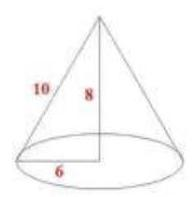
\includegraphics[max width=0.2\textwidth]{images/bo_d7ci9kqlb0pc73de9leg_1_668_1379_193_197_0.jpg}
\end{center}
\hspace*{3em} 

6. 已知函数 \(y = \left\{  \begin{array}{l} x\left( {x - b}\right) ,x \geq  0, \\  x\left( {{bx} + 1}\right) ,x < 0. \end{array}\right.\) 是奇函数,则 \(b = \_  - 1\) \_\_\_\_\_.

令 \(x > 0\) ,则 \(- x < 0\)

\(y\left( {-x}\right)  =  - y\left( x\right)\) 对 \(\forall x \in  \mathbf{R}\) 恒成立

\(- x\left( {-{bx} + 1}\right)  =  - x\left( {x - b}\right)\)

\(b{x}^{2} - x =  - {x}^{2} + {bx}\)

\(\left( {1 + b}\right) {x}^{2} - \left( {1 + b}\right) x = 0\)

\(\therefore b =  - 1\)

7. 某食品厂生产一种零食,该种零食每袋的质量 \(X\) (单位: \(\mathrm{g}\) ) 服从正态分布 \(N\left( {{65},{2.2}^{2}}\right)\) ,记作 \(X \sim  N\left( {{65},{2.2}^{2}}\right)\) . 规定: 这种零食的质量在 \({62.8} \sim  {69.4}\mathrm{\;g}\) 之间的为合格品; 则这种零食的合格率为\_\_\_\_\_0.819\_\_\_\_\_. (结果精确到 0.001)

参考数据: 若 \(X \sim  N\left( {\mu ,{\sigma }^{2}}\right)\) ,则 \(P\left( {\mu  - \sigma  \leq  X \leq  \mu  + \sigma }\right)  \approx  {0.6827},P\left( {\mu  - {2\sigma } \leq  X \leq  \mu  + {2\sigma }}\right)  \approx  {0.9545}\) , \(P\left( {\mu  - {3\sigma } \leq  X \leq  \mu  + {3\sigma }}\right)  \approx  {0.9973}.\)

\begin{center}
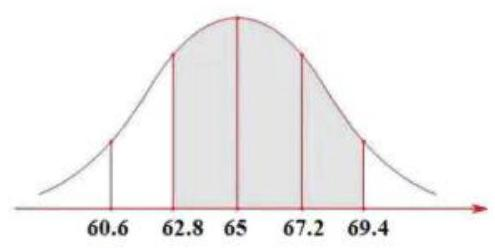
\includegraphics[max width=0.3\textwidth]{images/bo_d7ci9kqlb0pc73de9leg_2_1139_660_495_248_0.jpg}
\end{center}
\hspace*{3em} 

\(\mu  = {65},\;\sigma  = {2.2}\)

\(P\left( {{65} - {2.2} \leq  X \leq  {65} + {2.2}}\right)  = P\left( {{62.8} \leq  X \leq  {67.2}}\right)  \approx  {0.6827} \; P\left( {{65} - 2 \times  {2.2} \leq  X \leq  {65} + 2 \times  {2.2}}\right)  = P\left( {{60.6} \leq  X \leq  {69.4}}\right)  \approx  {0.9545} \; P\left( {{62.8} \leq  X \leq  {69.4}}\right)  = \frac{{0.9545} - {0.6827}}{2} + {0.6827} = {0.8186} \approx  {0.819}\)

8. 点 \(F\) 为抛物线 \(C : {y}^{2} = {8x}\) 的焦点， \(P\) 为 \(C\) 上一点，若 \(\bigtriangleup {POF}\) 的面积为 \(4\sqrt{2}\) ( \(O\) 为坐标原点)，则 \(\left| {PF}\right|  =\) \_\_\_\_\_6\_\_\_\_\_.

\begin{center}
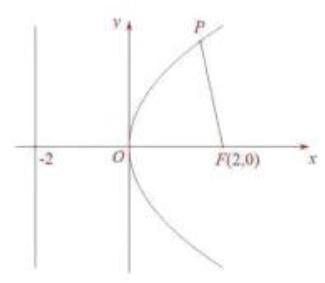
\includegraphics[max width=0.2\textwidth]{images/bo_d7ci9kqlb0pc73de9leg_2_856_1169_325_283_0.jpg}
\end{center}
\hspace*{3em} 

\({S}_{\bigtriangleup {POF}} = \frac{1}{2}{OF} \cdot  \left| {y}_{0}\right|  = 4\sqrt{2},{OF} = 2\)

\(\left| {y}_{0}\right|  = 4\sqrt{2},{x}_{0} = \frac{{y}_{0}^{2}}{8} = \frac{{16} \times  2}{8} = 4\)

\({PF} = {x}_{0} + 2 = 6\)

9. 从 6 名男生和 4 名女生中选出 3 人参加人工智能技能培训. 设事件 \(A\) : 至少抽到一名女生,事件 \(B\) : 恰好抽到一名男生,则 \(P\left( {B \mid  A}\right)  = \_ {0.36}\) \_.

\(P = \frac{{C}_{6}^{1}{C}_{4}^{2}}{{C}_{10}^{3} - {C}_{6}^{3}} = {0.36}\)

10. 已知复数 \(z = \cos \theta  + \mathrm{i}\sin \theta ,\theta  \in  \lbrack 0,{2\pi }),\mathrm{i}\) 是虚数单位,则 \({\left| z + 6\right| }^{2} + {\left| z - 8\mathrm{i}\right| }^{2}\) 的取值范围是\_\_\_\_\_ \(\left\lbrack  {{82},{122}}\right\rbrack\) \_\_\_\_\_. \(Z\left( {\cos \theta ,\sin \theta }\right)  = \left( {x,y}\right) ,{x}^{2} + {y}^{2} = 1\)

\({\left| z + 6\right| }^{2} + {\left| z - 8i\right| }^{2} = {\left( x + 6\right) }^{2} + {y}^{2} + {x}^{2} + {\left( y - 8\right) }^{2} = {12x} - {16y} + {102} \; = {12}\cos \theta  - {16}\sin \theta  + {102} = {20}\sin \left( {\theta  + \varphi }\right)  + {102} \in  \left\lbrack  {{82},{122}}\right\rbrack\)

11. 如图所示, \(A,B,C\) 为山脚两侧共线的三点,在山顶 \(P\) 处测得三点的俯角分别为 \(\alpha  = {29.3}^{ \circ  }\) ,

\(\beta  = {38.2}^{ \circ  },\gamma  = {25.1}^{ \circ  }\) . 计划沿直线 \({AC}\) 开通穿山隧道,为了求出隧道 \(\overset{\text{ ⏜ }}{DE}\) 的长度,还测得 \({AD} = {277}\) 米, \({BE} = {49}\) 米， \({BC} = {320}\) 米，则根据以上数据，隧道 \({DE}\) 的长度约为\_\_\_\_\_805\_\_\_\_\_米.(结果精确到 1 米)

\begin{center}
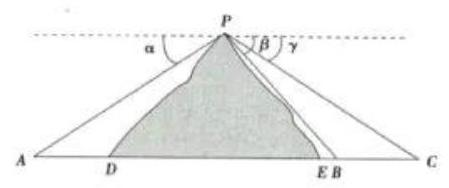
\includegraphics[max width=0.3\textwidth]{images/bo_d7ci9kqlb0pc73de9leg_3_173_346_449_188_0.jpg}
\end{center}
\hspace*{3em} 

过点 \(P\) 作 \({PH} \bot  {AC}\) 于点 \(H\)

在 \(\bigtriangleup {PBC}\) 中, \(\frac{320}{\sin \left( {\beta  - \gamma }\right) } = \frac{PB}{\sin \gamma }\)

\(\frac{320}{\sin \left( {{38.2}^{ \circ  } - {25.1}^{ \circ  }}\right) } = \frac{PB}{\sin {25.1}^{ \circ  }},\;{PB} \approx  {598.91}\)

在 \(\bigtriangleup {PHB}\) 中, \(\sin \beta  = \frac{PH}{PB}\)

\({PH} = {PB}\sin \beta  = {598.91}\sin {38.2}^{ \circ  } \approx  {370.371}\)

\(\tan \beta  = \frac{PH}{HB},\;{HB} = \frac{PH}{\tan \beta } = \frac{370.371}{\tan {38.2}^{ \circ  }} \approx  {470.658}\)

在 \(\bigtriangleup {PHA}\) 中, \(\tan \alpha  = \frac{PH}{AH},{AH} = \frac{PH}{\tan \alpha } = \frac{370.371}{\tan {29.3}^{ \circ  }} = {659.993}\)

\({DE} = {AB} - {AD} - {BE} = {AH} + {BH} - {AD} - {BE} = {659.993} + {470.658} - {277} - {49} \approx  {805}\) 米

12. 在平面直角坐标系 \({xOy}\) 中,点 \(A\left( {\cos \theta ,\sin \theta }\right) ,B\left( {-\sin \theta ,\cos \theta }\right) ,\theta  \in  \lbrack 0,{2\pi })\) . 若点 \(P\left( {x,y}\right)\) 满足: \(\overrightarrow{OP} \cdot  \overrightarrow{OA} = 1,\overrightarrow{OP} \cdot  \overrightarrow{OB} = 2\) ,则 \({xy}\) 的最大值是 \(- \frac{5}{2}\) .

\(\overrightarrow{OA} \cdot  \overrightarrow{OB} =  - \cos \theta \sin \theta  + \sin \theta \cos \theta  = 0\)

\begin{center}
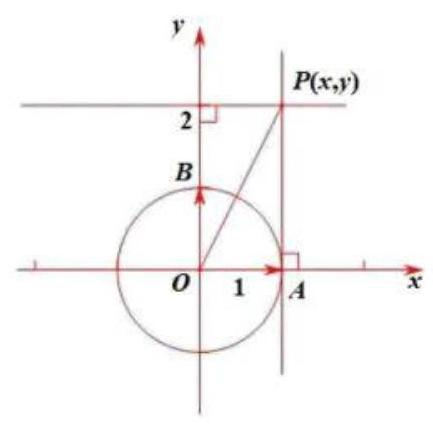
\includegraphics[max width=0.3\textwidth]{images/bo_d7ci9kqlb0pc73de9leg_3_1191_1585_433_425_0.jpg}
\end{center}
\hspace*{3em} 

\(\therefore {OA} \bot  {OB}\)

且 \(\left| \overrightarrow{OA}\right|  = \left| \overrightarrow{OB}\right|  = 1\)

\(\because \overrightarrow{OP} \cdot  \overrightarrow{OA} = 1,\overrightarrow{OP} \cdot  \overrightarrow{OB} = 2\)

\(\therefore \overrightarrow{OP}\) 在 \(\overrightarrow{OA}\) 上的数量投影为 \(1,\overrightarrow{OP}\) 在 \(\overrightarrow{OB}\) 上的数量投影为 2

\(\therefore {OP} = \sqrt{{1}^{2} + {2}^{2}} = \sqrt{5}\)

\(\therefore P\left( {\sqrt{5}\cos \alpha ,\sqrt{5}\sin \alpha }\right) \; {xy} = 5\sin \alpha \cos \alpha  = \frac{5}{2}\sin {2\alpha }\)

\({\left( xy\right) }_{\max } = \frac{5}{2}\)

\section*{二、选择题(本题共 4 小题，13-14 每小题 4 分，15-16 每小题 5 分，共 18 分. 在每小题给出的 四个选项中, 只有一项是符合题目要求的.)}

13. 已知 \(a > b > 0 > c\) ,则下列不等式成立的是(D)

A. \(\frac{c}{a} < \frac{c}{b}\) B. \(\frac{b}{a} > \frac{a}{b}\) C. \(\frac{b - c}{a - c} < \frac{b}{a}\) D. \(\frac{2}{a} + b < \frac{2}{b} + a\)

对于 \(\mathrm{D},a > b > 0,\frac{2}{b} > \frac{2}{a}\)

\(\therefore a + \frac{2}{b} > b + \frac{2}{a}\) ,选 D

14. 已知双曲线的方程为 \({x}^{2} - \frac{{y}^{2}}{4} = \lambda\) ,则 \(\left( A\right)\)

A. 渐近线与 \(\lambda\) 无关 B. 实轴长与 \(\lambda\) 无关

C. 焦距与 \(\lambda\) 无关 D. 焦点与 \(\lambda\) 无关

15. 音乐, 是人类精神通过无意识计算而获得的愉悦享受, 1807 年法国数学家傅里叶发现代表任何周期性声音的公式是形如 \(y = A\sin {\omega x}\) 的简单正弦型函数之和,而且这些正弦型函数的频率都是其中一个最小频率的整数倍,比如用小提琴演奏的某音叉的声音图像是由下图 1,2,3 三个函数图像组成的,则小提琴演奏的该音叉的声音函数可以为 \(\left( \begin{array}{l} C \end{array}\right)\)

\begin{center}
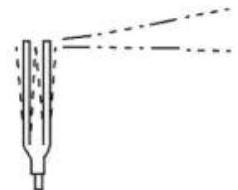
\includegraphics[max width=0.2\textwidth]{images/bo_d7ci9kqlb0pc73de9leg_4_154_1515_238_190_0.jpg}
\end{center}
\hspace*{3em} 

音叉

\begin{center}
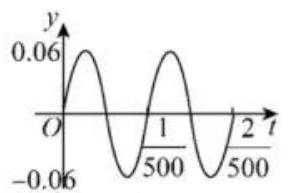
\includegraphics[max width=0.2\textwidth]{images/bo_d7ci9kqlb0pc73de9leg_4_399_1512_289_193_0.jpg}
\end{center}
\hspace*{3em} 

图1

\begin{center}
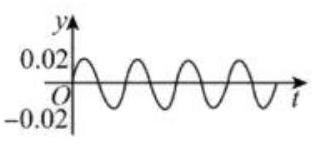
\includegraphics[max width=0.2\textwidth]{images/bo_d7ci9kqlb0pc73de9leg_4_702_1543_313_154_0.jpg}
\end{center}
\hspace*{3em} 

图2

\begin{center}
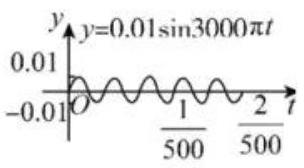
\includegraphics[max width=0.2\textwidth]{images/bo_d7ci9kqlb0pc73de9leg_4_1023_1537_304_168_0.jpg}
\end{center}
\hspace*{3em} 

图3

A. \(y = {0.06}\sin {1000\pi t} + {0.02}\sin {1500\pi t} + {0.01}\sin {3000\pi t}\)

B. \(y = {0.06}\sin {1000\pi t} + {0.02}\sin {2500\pi t} + {0.01}\sin {3000\pi t}\)

C. \(y = {0.06}\sin {1000\pi t} + {0.02}\sin {2000\pi t} + {0.01}\sin {3000\pi t}\)

D. \(y = {0.06}\sin {500\pi t} + {0.02}\sin {2000\pi t} + {0.01}\sin {3000\pi t}\)

\[
{\omega }_{1} = \frac{2\pi }{{T}_{1}} = \frac{2\pi }{\frac{1}{500}} = {1000\pi }
\]

\[
f = \frac{1}{T} = \frac{\omega }{2\pi }
\]

\(\because f\) 成整数倍

\(\therefore \omega\) 成整数倍,选 C

16. 已知函数 \(y = f\left( x\right)\) 的表达式为 \(f\left( x\right)  = \left( {x - 1}\right) \left( {x - a}\right) \left( {x - b}\right) ,x \in  \mathbf{R}\) ,则下列命题正确的是(B)

A. 函数 \(y = f\left( x\right)\) 的零点的个数一定是 3 个

B. 若集合 \(A = \{ x \mid  f\left( x\right)  \geq  0\}\) 的解集是 \(\lbrack 0, + \infty )\) ,则实数对 \(\left( {a,b}\right)\) 有 2 对

C. 函数 \(y = f\left( x\right)\) 必存在极值

D. 函数 \(y = f\left( x\right)\) 在 \(\left( {b,0}\right)\) 处的切线方程为 \(y = 0\) ,则 \(b = 1\)

\begin{center}
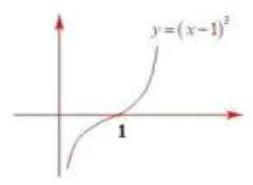
\includegraphics[max width=0.2\textwidth]{images/bo_d7ci9kqlb0pc73de9leg_5_722_994_253_185_0.jpg}
\end{center}
\hspace*{3em} 

对于 \(\mathrm{A}\text{ 、 }\mathrm{C}\) ,当 \(a = b = 1\) 时,

\(f\left( x\right)  = {\left( x - 1\right) }^{3}\) 只有 1 个零点

无极值, \(\mathrm{A}\text{ 、 }\mathrm{C}\) 错误

\begin{center}
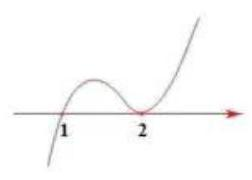
\includegraphics[max width=0.2\textwidth]{images/bo_d7ci9kqlb0pc73de9leg_5_726_1202_252_180_0.jpg}
\end{center}
\hspace*{3em} 

对于 \(\mathrm{D}\) ,当 \(a = b = 2\) 时,

\(f\left( x\right)  = \left( {x - 1}\right) {\left( x - 2\right) }^{2}\)

其切线也为 \(y = 0\)

\begin{center}
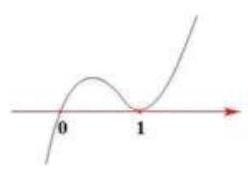
\includegraphics[max width=0.2\textwidth]{images/bo_d7ci9kqlb0pc73de9leg_5_737_1433_248_174_0.jpg}
\end{center}
\hspace*{3em} 

对于 \(B\) ,如图, \(f\left( x\right)  = x{\left( x - 1\right) }^{2}\)

则 \(a = 0,b = 1\) 或 \(a = 1,b = 0\)

2 对, B 正确, 选 B

\section*{三、解答题(本题共 5 小题，17-19 题每题 14 分，20-21 题每题 18 分，共 78 分. 解答应写出文 字说明, 证明过程或演算步骤.)}

17. 已知函数 \(y = f\left( x\right)\) 的表达式为 \(f\left( x\right)  = \sin \left( {{\pi x} + \varphi }\right) ,\left( {-\frac{\pi }{2} < \varphi  < \frac{\pi }{2}}\right)\) .

(1) \(f\left( 0\right)  = \frac{3}{5}\) ，求 \(f\left( \frac{1}{4}\right)\) 的值；

(2)若 \(f\left( \frac{1}{2}\right) ,f\left( 1\right) ,f\left( 2\right)\) 依次成等比数列,求 \(\varphi\) 的值.

(1) \(f\left( 0\right)  = \sin \varphi  = \frac{3}{5},\;\varphi  \in  \left( {-\frac{\pi }{2},\frac{\pi }{2}}\right) ,\cos \varphi  = \frac{4}{5}\)

\(f\left( \frac{1}{4}\right)  = \sin \left( {\frac{\pi }{4} + \varphi }\right)  = \sin \frac{\pi }{4}\cos \varphi  + \cos \frac{\pi }{4}\sin \varphi  = \frac{\sqrt{2}}{2}\left( {\frac{3}{5} + \frac{4}{5}}\right)  = \frac{7\sqrt{2}}{10}\)

(2) \({f}^{2}\left( 1\right)  = f\left( \frac{1}{2}\right)  \cdot  f\left( 2\right)\)

\({\sin }^{2}\left( {\pi  + \varphi }\right)  = \sin \left( {\frac{\pi }{2} + \varphi }\right)  \cdot  \sin \left( {{2\pi } + \varphi }\right)\)

\({\sin }^{2}\varphi  = \cos \varphi \sin \varphi ,\varphi  \in  \left( {-\frac{\pi }{2},\frac{\pi }{2}}\right) ,\sin \varphi  \neq  0,\cos \varphi  \neq  0\)

\(\sin \varphi  = \cos \varphi\)

\(\tan \varphi  = 1,\;\varphi  = \frac{\pi }{4}\)

18. 某工厂生产的某种产品的月产量(单位:千件)与单位成本(单位:元/件)的数据如下:

\begin{center}
\adjustbox{max width=\textwidth}{
\begin{tabular}{|c|c|c|}
\hline
月份 & 产量 \(\;x\) (千件) & 单位成本 \(y\) (元/件) \\
\cline{1-3}
1 & 2 & 73 \\
\cline{1-3}
2 & 3 & 72 \\
\cline{1-3}
3 & 4 & 71 \\
\cline{1-3}
4 & 3 & 73 \\
\cline{1-3}
5 & 4 & 69 \\
\cline{1-3}
6 & 5 & 68 \\
\cline{1-3}
\hline
\end{tabular}
}
\end{center}

(1)计算产量与单位成本的相关系数(无需过程);

(2)建立产量与单位成本的回归方程(写出必要的过程)；

(3)若该工厂计划 7 月份生产 7 千件该产品，则单位成本预计是多少？

附:相关系数 \(r\) 的计算公式: \(r = \frac{\mathop{\sum }\limits_{{i = 1}}^{n}\left( {{x}_{i} - \overline{x}}\right) \left( {{y}_{i} - \overline{y}}\right) }{\sqrt{\mathop{\sum }\limits_{{i = 1}}^{n}{\left( {x}_{i} - \overline{x}\right) }^{2}\mathop{\sum }\limits_{{i = 1}}^{n}{\left( {y}_{i} - \overline{y}\right) }^{2}}}\) ;

回归系数计算公式: \(\left\{  \begin{array}{l} \widehat{a} = \frac{\mathop{\sum }\limits_{{i = 1}}^{n}\left( {{x}_{i} - \bar{x}}\right) \left( {{y}_{i} - \bar{y}}\right) }{\mathop{\sum }\limits_{{i = 1}}^{n}{\left( {x}_{i} - \bar{x}\right) }^{2}} = \frac{\mathop{\sum }\limits_{{i = 1}}^{n}{x}_{i}{y}_{i} - n\overline{xy}}{\mathop{\sum }\limits_{{i = 1}}^{n}{x}_{i}^{2} - n{\bar{x}}^{2}}, \\  \widehat{b} = \bar{y} - \widehat{a}\bar{x} = \frac{\mathop{\sum }\limits_{{i = 1}}^{n}{y}_{i} - \widehat{a}\mathop{\sum }\limits_{{i = 1}}^{n}{x}_{i}}{n}. \end{array}\right.\)

(1) \(r =  - \frac{10}{11}\)

(2)设 \(\widehat{y} = \widehat{a}x + \widehat{b}\)

代入公式 (实际用计算器),得 \(\widehat{a} =  - \frac{20}{11},\widehat{b} = \frac{851}{11}\)

\(\therefore \widehat{y} =  - \frac{20}{11}x + \frac{851}{11}\)

(3) \(y\left( 7\right)  =  - \frac{20}{11} \times  7 + \frac{851}{11} = \frac{711}{11}\)

19. 在四棱锥 \(P - {ABCD}\) 中,四边形 \({ABCD}\) 是菱形, \({PA} = {PC} = 5,{PB} = {PD} = 2\sqrt{5},{AC} = 6\) ,点 \(F\) 为 \({PD}\) 的中点,点 \(E\) 为 \({PB}\) 上的点, \(\overline{PE} = \lambda \overline{PB},\lambda  \in  \left( {0,1}\right)\) ,平面 \({AFE}\) 与棱 \({PC}\) 交于点 \(G\) .

\begin{center}
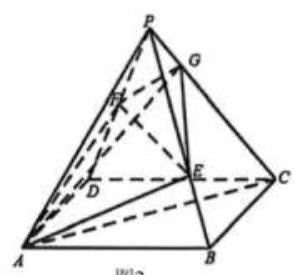
\includegraphics[max width=0.2\textwidth]{images/bo_d7ci9kqlb0pc73de9leg_7_520_1216_300_275_0.jpg}
\end{center}
\hspace*{3em} 

图2

\begin{center}
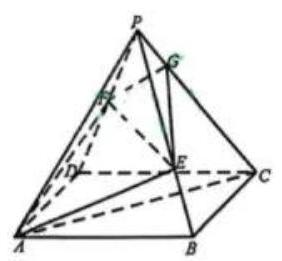
\includegraphics[max width=0.2\textwidth]{images/bo_d7ci9kqlb0pc73de9leg_7_153_1216_282_261_0.jpg}
\end{center}
\hspace*{3em} 

图1

(1)求证:异面直线 \({EF}\) 与 \({AC}\) 垂直；

(2)当 \(\lambda  = \frac{2}{3}\) 时,求 \({AG}\) 与底面 \({ABCD}\) 所成的线面角大小.

(1)连接 \({BD}\) 交 \({AC}\) 于点 \(O\)

\(\because {PA} = {PC},{PB} = {PD},O\) 为 \({AC}\text{ 、 }{BD}\) 中点

\(\therefore {PO} \bot  {AC},{PO} \bot  {BD}\)

\(\because {AC} \cap  {BD} = O,{AC} \subset\) 平面 \({ABCD},{BD} \subset\) 平面 \({ABCD}\)

\(\therefore {PO} \bot\) 平面 \({ABCD}\)

\(\therefore {EF}\) 在平面 \({ABCD}\) 的投影为 \({BD}\)

在菱形 \({ABCD}\) 中, \({AC} \bot  {BD}\)

\(\therefore {AC} \bot  {EF}\)

(2) \({PA} = {PC} = 5,\;{AO} = \frac{1}{2}{AC} = 3\)

\({PO} = \sqrt{{5}^{2} - {3}^{2}} = 4,\;{PB} = {PD} = 2\sqrt{5}\)

\({OD} = {OB} = \sqrt{{\left( 2\sqrt{5}\right) }^{2} - {4}^{2}} = 2\)

\begin{center}
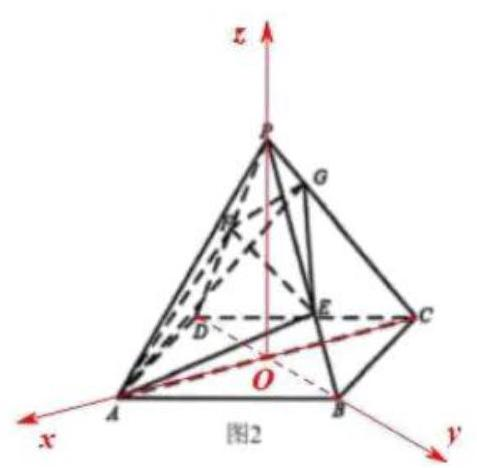
\includegraphics[max width=0.3\textwidth]{images/bo_d7ci9kqlb0pc73de9leg_8_1071_654_477_468_0.jpg}
\end{center}
\hspace*{3em} 

如图建系, \(A\left( {3,0,0}\right) ,C\left( {-3,0,0}\right) ,P\left( {0,0,4}\right)\) ,

\(B\left( {0,2,0}\right) ,\;D\left( {0, - 2,0}\right)\)

\(F\) 为 \({PD}\) 中点, \(F\left( {0, - 1,2}\right)\)

\[
\overrightarrow{PE} = \lambda \overrightarrow{PB} = \lambda \left( {0,2, - 4}\right)  = \frac{2}{3}\left( {0,2, - 4}\right)  = \left( {0,\frac{4}{3}, - \frac{8}{3}}\right)
\]

\(\left( {{x}_{E},{y}_{E},{z}_{E} - 4}\right)  = \left( {0,\frac{4}{3}, - \frac{8}{3}}\right)\)

\[
\therefore E\left( {0,\frac{4}{3},\frac{4}{3}}\right)
\]

\(\overrightarrow{PG} = t\overrightarrow{PC} = t\left( {-3,0, - 4}\right)  = \left( {-{3t},0, - {4t}}\right)\)

\(\left( {{x}_{G},{y}_{G},{z}_{G} - 4}\right)  = \left( {-{3t},0, - {4t}}\right)\)

\(\therefore G\left( {-{3t},0,4 - {4t}}\right) ,\overrightarrow{AG} = \left( {-{3t} - 3,0,4 - {4t}}\right)\)

设平面 \({AEF}\) 的一个法向量为 \(\overrightarrow{n} = \left( {x,y,z}\right)\)

则 \(\left\{  \begin{array}{l} \overrightarrow{n} \cdot  \overrightarrow{AE} =  - {3x} + \frac{4}{3}y + \frac{4}{3}z = 0 \\  \overrightarrow{n} \cdot  \overrightarrow{AF} =  - {3x} - y + {2z} = 0 \end{array}\right.\)

令 \(x = 4\) ,得 \(y = 2,z = 7,\overrightarrow{n} = \left( {4,2,7}\right)\)

\(\overrightarrow{n} \cdot  \overrightarrow{AG} = 4\left( {-{3t} - 3}\right)  + 7\left( {4 - {4t}}\right)  = 0,\;t = \frac{2}{5}\)

\[
\overrightarrow{AG} = \left( {-\frac{21}{5},0,\frac{12}{5}}\right)
\]

易知平面 \({ABCD}\) 的一个法向量 \(\overrightarrow{m} = \left( {0,0,1}\right)\)

则 \(\sin \theta  = \frac{\left| \overrightarrow{AG} \cdot  \overrightarrow{m}\right| }{\left| \overrightarrow{AG}\right| \left| \overrightarrow{m}\right| } = \frac{\frac{12}{5}}{\sqrt{{\left( \frac{21}{5}\right) }^{2} + {\left( \frac{12}{5}\right) }^{2}}} = \frac{4\sqrt{65}}{65}\)

\(\therefore \theta  = \arcsin \frac{4\sqrt{65}}{65}\)

20. 已知椭圆 \(\Gamma  : \frac{{x}^{2}}{{a}^{2}} + \frac{{y}^{2}}{{b}^{2}} = 1\left( {a > b > 0}\right)\) 经过点 \(\left( {0,1}\right)\) ,离心率为 \(\frac{\sqrt{2}}{2}\) . 过点 \(M\left( {0, - m}\right) ,m > 0\) 的动直线 \(l\) 交椭圆 \(\Gamma\) 于 \(C,D\) 两点.

(1)求椭圆 \(\Gamma\) 的方程；

( 2 )若直线 \(l\) 与 \({x}^{2} + {y}^{2} = \frac{2}{3}\) 相切，求当 \(m = 2\) 时， \({CD}\) 的长；

(3)若以 \({CD}\) 为直径的圆经过 \(x\) 轴上方的定点 \(P\) ，求点 \(P\) 的坐标.

\begin{center}
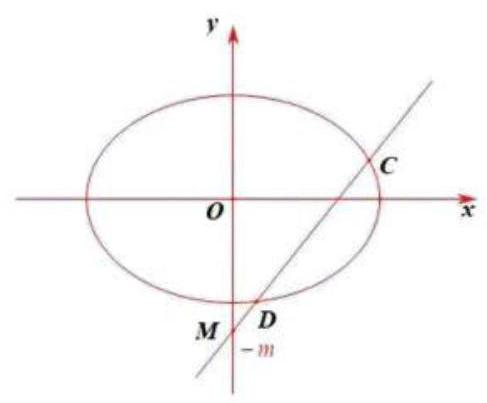
\includegraphics[max width=0.3\textwidth]{images/bo_d7ci9kqlb0pc73de9leg_9_928_1093_487_403_0.jpg}
\end{center}
\hspace*{3em} 

(1) \(b = 1,\frac{c}{a} = \frac{\sqrt{2}}{2},{a}^{2} = {b}^{2} + {c}^{2} = {c}^{2} + 1\)

\(\therefore {a}^{2} = 2,\frac{{x}^{2}}{2} + {y}^{2} = 1\)

(2)由题， \({k}_{l}\) 存在，设 \(l : y = {kx} - 2\)

\(d = \frac{2}{\sqrt{{k}^{2} + 1}} = \sqrt{\frac{2}{3}}\)

\({k}^{2} = 5\) ,由对称性,不妨取 \(k = \sqrt{5}\)

联立 \(\left\{  \begin{array}{l} y = {kx} - 2 \\  \frac{{x}^{2}}{2} + {y}^{2} = 1 \end{array}\right.\) ,得 \(\left( {1 + 2{k}^{2}}\right) {x}^{2} - {8kx} + 6 = 0\)

即 \({11}{x}^{2} - 8\sqrt{5}x + 6 = 0\)

\(\Delta  = {56},\;{CD} = \sqrt{1 + {k}^{2}} \cdot  \frac{\sqrt{56}}{11} = \frac{4\sqrt{21}}{11}\)

(3)设 \(P\left( {{x}_{0},{y}_{0}}\right) ,C\left( {{x}_{1},{y}_{1}}\right) ,D\left( {{x}_{2},{y}_{2}}\right)\) ，当 \(k\) 存在时

联立 \(\left\{  \begin{array}{l} y = {kx} - m \\  \frac{{x}^{2}}{2} + {y}^{2} = 1 \end{array}\right.\) ,得 \(\left( {1 + 2{k}^{2}}\right) {x}^{2} - {4kmx} + 2\left( {{m}^{2} - 1}\right)  = 0\)

\(\Delta  > 0,\;{x}_{1} + {x}_{2} = \frac{4km}{1 + 2{k}^{2}},\;{x}_{1}{x}_{2} = \frac{2\left( {{m}^{2} - 1}\right) }{1 + 2{k}^{2}}\)

\({y}_{1} + {y}_{2} = k{x}_{1} - m + k{x}_{2} - m = k\left( {{x}_{1} + {x}_{2}}\right)  - {2m} = \frac{-{2m}}{1 + 2{k}^{2}}\)

\({y}_{1}{y}_{2} = \left( {k{x}_{1} - m}\right) \left( {k{x}_{2} - m}\right)  = {k}^{2}{x}_{1}{x}_{2} - {km}\left( {{x}_{1} + {x}_{2}}\right)  + {m}^{2} = \frac{{m}^{2} - 2{k}^{2}}{1 + 2{k}^{2}}\)

由题, \(\overrightarrow{PC} \cdot  \overrightarrow{PD} = 0\)

\[
\overrightarrow{PC} \cdot  \overrightarrow{PD} = \left( {{x}_{1} - {x}_{0},{y}_{1} - {y}_{0}}\right)  \cdot  \left( {{x}_{2} - {x}_{0},{y}_{2} - {y}_{0}}\right)  = \left( {{x}_{1} - {x}_{0}}\right)  \cdot  \left( {{x}_{2} - {x}_{0}}\right)  + \left( {{y}_{1} - {y}_{0}}\right)  \cdot  \left( {{y}_{2} - {y}_{0}}\right)
\]

\[
= {x}_{1}{x}_{2} - {x}_{0}\left( {{x}_{1} + {x}_{2}}\right)  + {x}_{0}^{2} + {y}_{1}{y}_{2} - {y}_{0}\left( {{y}_{1} + {y}_{2}}\right)  + {y}_{0}^{2} = 0
\]

代入韦达定理,得 \(\left( {2{x}_{0}^{2} + 2{y}_{0}^{2} - 2}\right) {k}^{2} - {4m}{x}_{0}k + 3{m}^{2} - 2 + {x}_{0}^{2} + {2m}{y}_{0} + {y}_{0}^{2} = 0\)

若对 \(\forall \mathbf{k}\) 恒成立,则

\[
\left\{  \begin{array}{l} 2{x}_{0}^{2} + 2{y}_{0}^{2} - 2 = 0,{y}_{0} > 0 \\   - {4m}{x}_{0} = 0,m > 0 \\  3{m}^{2} - 2 + {x}_{0}^{2} + {2m}{y}_{0} + {y}_{0}^{2} = 0 \end{array}\right.
\]

\(\therefore {x}_{0} = 0,{y}_{0} = 1\) ,此时, \(3{m}^{2} + {2m} - 1 = 0,m = \frac{1}{3}\)

当 \(k\) 不存在时, \({x}^{2} + {y}^{2} = 1\) 过 \(\left( {0,1}\right)\)

\(\therefore\) 定点为 \(P\left( {0,1}\right)\)

21. 设定义域为 \(\left( {0, + \infty }\right)\) 的函数 \(y = f\left( x\right)\) 的表达式为 \(f\left( x\right)  = {e}^{x} - a\left( {a > 0}\right)\) ,我们可以证明函数 \(y = f\left( x\right)\) 存在唯一的零点,设该零点为 \(r\) .

如图,过点 \({A}_{1}\left( {{x}_{1},f\left( {x}_{1}\right) }\right)\) 作函数 \(y = f\left( x\right)\) 的切线 \({l}_{1}\) 与 \(x\) 轴的交点为 \({B}_{2}\) ,设横坐标为 \({x}_{2}\) ,若 \({x}_{2} > r\) ,则过点 \({A}_{2}\left( {{x}_{2},f\left( {x}_{2}\right) }\right)\) 作函数 \(y = f\left( x\right)\) 的切线 \({l}_{2}\) 与 \(x\) 轴的交点为 \({B}_{3}\) ,设横坐标为 \({x}_{3}\) ; 若 \({x}_{2} \leq  r\) ,则停止作切线.

\begin{center}
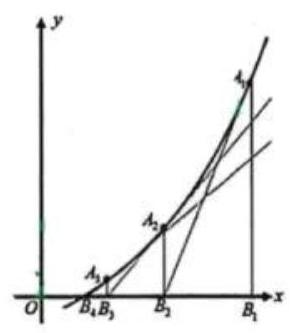
\includegraphics[max width=0.2\textwidth]{images/bo_d7ci9kqlb0pc73de9leg_11_1326_532_294_333_0.jpg}
\end{center}
\hspace*{3em} 

依次类推,得到数列 \(\left\{  {x}_{n}\right\}  \left( {n \geq  1,n \in  \mathbf{N}}\right)\) ,记 \({x}_{1} = t,t > r\) .

(1)若 \(a = e,t = 2\) ，求 \({x}_{2}\) ；

(2)求证:数列 \(\left\{  {x}_{n}\right\}\) 是严格减数列；

(3)若 \(a = 1\) ，比较 \({x}_{n + 1} + 1\) 与 \({x}_{n} - \ln {x}_{n}\) 的大小，并说明理由.

(1) \(f\left( x\right)  = {e}^{x} - e,{x}_{1} = t = 2\)

\({A}_{1}\left( {2,{e}^{2} - e}\right) ,\;{f}^{\prime }\left( x\right)  = {e}^{x},\;k = {f}^{\prime }\left( 2\right)  = {e}^{2}\)

\({A}_{1}{B}_{2} : y - \left( {{e}^{2} - e}\right)  = {e}^{2}\left( {x - 2}\right)\)

令 \(y = 0,{x}_{2} = \frac{1}{e} + 1\)

(2) \({A}_{n}\left( {{x}_{n},f\left( {x}_{n}\right) }\right) ,\;f\left( {x}_{n}\right)  = {e}^{{x}_{n}} - a\)

\({f}^{\prime }\left( x\right)  = {e}^{x},\;k = {f}^{\prime }\left( {x}_{n}\right)  = {e}^{{x}_{n}}\)

\({A}_{n}{B}_{n + 1} : y - f\left( {x}_{n}\right)  = {e}^{{x}_{n}}\left( {x - {x}_{n}}\right)\)

令 \(y = 0, - f\left( {x}_{n}\right)  = {e}^{{x}_{n}}\left( {{x}_{n + 1} - {x}_{n}}\right)\)

\(a - {e}^{{x}_{n}} = {e}^{{x}_{n}}\left( {{x}_{n + 1} - {x}_{n}}\right)\)

\({x}_{n + 1} - {x}_{n} = \frac{a}{{e}^{{x}_{n}}} - 1\)

只要证 \({x}_{n + 1} - {x}_{n} < 0\)

即证 \(\frac{a}{{e}^{{x}_{n}}} - 1 < 0\)

即证 \(a < {e}^{{x}_{n}}\)

即证 \({x}_{n} > \ln a\)

由题, \(f\left( r\right)  = {e}^{r} - a = 0,r = \ln a\) 且 \({x}_{n} > r\)

得证

\begin{center}
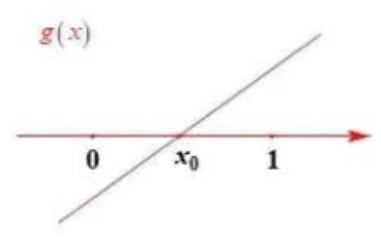
\includegraphics[max width=0.2\textwidth]{images/bo_d7ci9kqlb0pc73de9leg_12_1015_339_381_241_0.jpg}
\end{center}
\hspace*{3em} 

\(\therefore \left\{  {x}_{n}\right\}\) 严格减

(3) \(f\left( x\right)  = {e}^{x} - 1 = 0,x = 0\)

\(\therefore {x}_{n} > 0\)

由 (2) 得 \({x}_{n + 1} = {x}_{n} + \frac{a}{{e}^{{x}_{n}}} - 1 = {x}_{n} + \frac{1}{{e}^{{x}_{n}}} - 1\)

\({x}_{n + 1} + 1 - {x}_{n} + \ln {x}_{n} = {x}_{n} + \frac{1}{{e}^{{x}_{n}}} - {x}_{n} + \ln {x}_{n} = \frac{1}{{e}^{{x}_{n}}} + \ln {x}_{n}\)

令 \(g\left( x\right)  = \frac{1}{{e}^{x}} + \ln x,x > 0\)

\({g}^{\prime }\left( x\right)  =  - {e}^{-x} + \frac{1}{x} = \frac{1 - x{e}^{-x}}{x} = \frac{{e}^{x} - x}{x{e}^{x}}\)

易知,当 \(x > 0\) 时, \({e}^{x} > x\)

\(\therefore {g}^{\prime }\left( x\right)  > 0,g\left( x\right)\) 严格增

\(g\left( {0}^{ + }\right)  =  - \infty ,\;g\left( 1\right)  = \frac{1}{e} > 0,\;\exists {x}_{0} \in  \left( {0,1}\right)\) 使得 \(g\left( {x}_{0}\right)  = 0\)

\(\therefore\) 当 \({x}_{n} \geq  {x}_{0}\) 时, \(g\left( x\right)  \geq  0,{x}_{n + 1} + 1 \geq  {x}_{n} - \ln {x}_{n}\)

当 \({x}_{n} < {x}_{0}\) 时, \(g\left( x\right)  < 0,{x}_{n + 1} + 1 < {x}_{n} - \ln {x}_{n}\)

中国大陆 上海

\begin{center}

\includegraphics[max width=1.0\textwidth]{images/bo_d7ci9kqlb0pc73de9leg_13_53_481_1788_1824_0.jpg}
\end{center}
\hspace*{3em} 

\end{document}